\section{Dynamic Resource Exchange}\label{abm:dre}

Dynamic Resource Exchange (DRE) is the functional bedrock on which Cyclus
simulations are built. It defines the interaction mechanisms and methodolgies
for agents, specifically agents whose archetypes have implemented the
\code{Trader} interface. This section begins by providing a motivating problem
statement in \S \ref{abm:dre:prob}. It then details the methodology for querying
supply and demand during the information gathering phase of the DRE in \S
\ref{abm:dre:info}. The solution phase, in which the defined DRE is translated
into a form of the Multicommodity Transportation Problem (MCTP) and solved, is
then described in \S \ref{abm:dre:fctp}. Finally, two proof of principle
simulations with novel fuel cycle DREs are presented in \S \ref{abm:dre:proof}.

\subsection{Problem Statement}\label{abm:dre:prob}

As a next-generation nuclear fuel cycle simulation framework, Cyclus maintains a
primary goal of modeling flexibility. As facility, institutional, and regional
archetypes are proposed, they should be relatively easily implemented and
utilized in the Cyclus simulation framework. Furthermore, the level of modeling
abstraction for different facilities in a fuel cycle will be different based on
the needs of archetype developer. Any supply-demand resolution framework,
therefore, must be able to support arbitrary facilities. One way to approach
such a problem is to treat facilities as black boxes, clearly defining a
supply-demand communication framework.

As stated previously in \S \ref{abm:abm:limits}, a number of considerations must
be taken into account in such a framework. Supply and demand must be able to be
solved globally at any given time step. Resources must be able to be treated in
a fungible manner. The framework must be able to incorporate arbitrary,
agent-defined constraints.

In order to address each of these concerns, the concept of a Dynamic Resource
Exchange (DRE) was developed and implemented. That process was motivated by the
following problem statement:

\begin{quote}
    If facilities are treated as individual black boxes and connections between
    facilities are determined dynamically, how does one match suppliers with
    consumers considering quantity and quality-based supply constraints,
    quantity and quality-based demand constraints, supply response to
    quality-based demands, and issues of fungibility?
\end{quote}

\subsection{Information Gathering}\label{abm:dre:info}

Supply-demand determination at any given time step begins with three
\textit{phases}, the terminology of which is influenced from previous supply
chain agent-based modeling work \cite{julka_agent-based_2002}. Importantly, this
information-gathering step is agnostic as to the supply-demand matching
algorithm used, it is concerned only with querying the current status of supply
and demand in the simulation. The collective information gathering procedure is
shown in Figure \ref{fig:procedure}.

\begin{figure}
  \begin{center}
    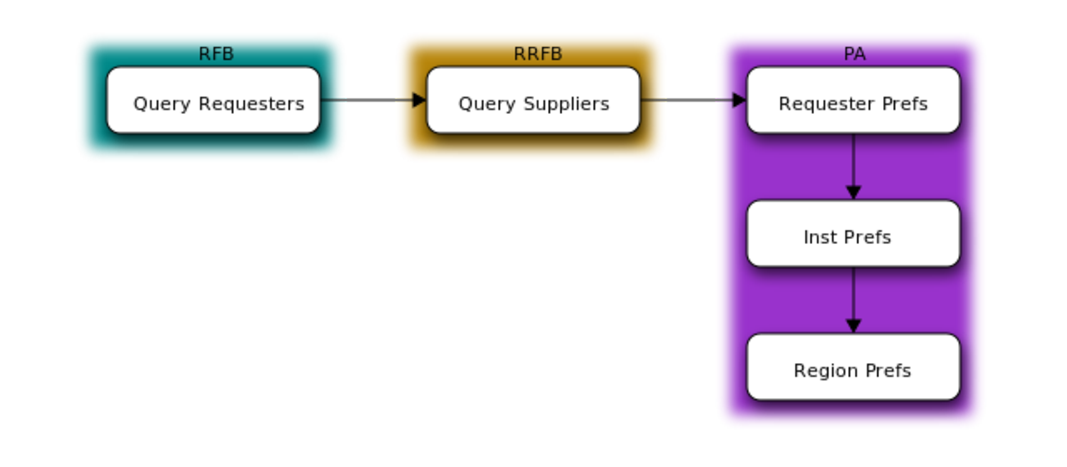
\includegraphics[]{./figs/procedure.pdf}
    \caption[]{\label{fig:procedure}
        Schematic illustrating the DRE's information gathering procedure.}
  \end{center}
\end{figure}

The first phase allows consumers of commodities to denote both the quantity of a
commodity they need to consume as well as the target isotopics, or quality, by
\textit{posting} their demand to the market exchange. This posting informs
producers of commodities what is needed by consumers, and is termed the
\textit{Request for Bids} (RFB) phase. Consumers are allowed to over-post, i.e.,
request more quantity than they can actually consume, as long as a corresponding
capacity constraint accompanies this posting. Requests can be denoted as
\textit{exclusive}. An exclusive request is one that must either be met in full
or not at all. Exclusive requests allow the modeling of quantized, packaged
transfers, e.g., fuel assemblies. Further, consumers are allowed to post demand
for multiple commodities that may serve to meet the same combine capacity. For
example, consider an LWR that can be filled with MOX or UOX. It can post a
demand for both, but must define a preference over the set of possible
commodities that can be consumed. Such requests are termed \textit{mutual
  requests}. Another example is that of an advanced fuel fabrication facility,
i.e., one that fabricates fuel partially from separated material that has
already passed through a reactor. Such a facility can choose to fill the
remaining space in a certain assembly with various types of fertile material,
including depleted uranium from enrichment or reprocessed uranium from
separations. Accordingly, it could demand both commodities as long as it
provides a corresponding constraint with respect to total consumption. At the
completion of the RFB phase, the market exchange will have a set of request
portfolios. Each each portfolio consists of a set requests. Arbitrary
constraints over the set of requests can be provided that are functions of
quantity or quality.  For requests that mutually satisfy a given demand, a
preference over those requests is required. Finally, each request portfolio has
a specific quantity associated with it.

The second phase allows suppliers to \textit{respond} to the set of request
portfolios, and is termed the \textit{Response to Request for Bids} (RRFB) phase
(analogous to Julka's Reply to Request for Quote phase
\cite{julka_agent-based_2002}). Each request portfolio is comprised of requests
for some set of commodities. Accordingly, for each request, suppliers of that
commodity denote production capacities and an isotopic profile of the commodity
they can provide. Suppliers are allowed to offer the null set of isotopics as
their profile, effectively providing no information. Suppliers are also allowed
to denote responses as \textit{exclusive}, as is done in the RFB phase. An
exclusive offer must be accepted in its entirety or not at all. Again, exclusive
offers provides a way to model quantized, packaged resources, such as fuel
assemblies. A supplier may have its production constrained by more than one
parameter. For example, a processing facility may have both a throughput
constraint (i.e., it can only process material at a certain rate) and an
inventory constraint (i.e., it can only hold some total material). Further, the
facility could have a constraint on the quality of material to be processed,
e.g., it may be able to handle a maximum radiotoxicity for any given time step
which is a function of both the quantity of material in processes and the
isotopic content of that material. Multiple of such constraints are allowed. At
the completion of the RRFB phase the possible connections between supplier and
producer facilities, i.e., the arcs in the graph of the transportation problem,
have been established with specific capacity constraints defined both by the
quantity and quality of commodities that will traverse the arcs.

The final phase of the information gathering procedure allows consumer
facilities to adjust their set of preferences and for managers of consumer
facilities to affect the consumer's set of preferences, as described in the
remaining sections. Accordingly, the last phase is termed the \textit{Preference
 Adjustment} (PA) phase. Preference adjustments can occur in response to the
set of responses provided by producer facilities. Consider the example of a
reactor facility that requests two fuel types, MOX and UOX. It may get two
responses to its request for MOX, each with different isotopic profiles of the
MOX that can be provided. It can then assign preference values over this set of
potential MOX providers. Another prime example is in the case of repositories. A
repository may have a defined preference of material to accept based upon its
heat load or radiotoxicity, both of which are functions of the quality, or
isotopics, of a material. In certain simulators, limits on fuel entering a
repository are imposed based upon the amount of time that has elapsed since the
fuel has exited a reactor, which can be assessed during this phase. The time
constraint is, in actuality, a constraint on heat load or radiotoxicity (one
must let enough of the fission products decay). A repository could analyze
possible input fuel isotopics and set the arc preference of any that violate a
given rule to 0, effectively eliminating that arc.

\subsection{The Nuclear Fuel Cycle Transportation Problem}\label{abm:dre:fctp}

Supply and demand in a nuclear fuel cycle context is inherently a multicommodity
problem. A light water reactor can be fueled by both UOX and MOX fuel, for
instance. How it is fueled is a result both of fuel availability and associated
preferences. Allowing for complex physical and chemical constraints on both
processes and inventories, as well as including economics-based approaches for
determining exchange preferences is a complicated affair. Determining the
optimum solution to such a system is even more complicated. Accordingly,
sophisticated tools in both the operations research and agent based modeling
realms have been leveraged to accomplish the task.

An instance of supply and demand defined by the DRE information gathering step
can be solved in a variety of ways. It can be casted to a constrained, bipartite
network, and any heuristic that provides a feasible solution to such networks
are valid. To solve the system optimally, however, a formal investigation and
solution structure is needed. This section describes the construction of such a
formulation, entitled the \textit{Nuclear Fuel Cycle Transportation Problem}
(NFCTP).

The basis for the formulation is the Multicommodity Transportation Problem
described in \S\ref{intro:mtp} with some departures described in detail
below. Two separate formulations are provided. The first is a strictly linear
program (LP) while the second is a mixed-integer linear program (MILP). A
heuristic is also provided that provides a reasonable solution to most simple
problems.

The LP formulation can be solved quickly, but allows split orders. In other
words, the LP formulation solves a relaxation of the defined instance that does
not take into account \textit{exclusive} requests or bids. The nuclear fuel
cycle deals with bundled orders, such as nuclear fuel assemblies, thus this
modeling paradigm is only an approximation. The MILP provides a more realistic
exchange, but can take much longer to solve. 

\subsubsection{Terminology}

Objects and datastructures generated in the information gathering procedure are
used in the formal definition of the NFCTP and must be defined.

Each portfolio can be considered separately. The set of supply portfolios is
denoted as $S$ and the set of request portfolios is denoted as $R$. Each supply
portfolio is comprsied of $s_M$ supply nodes, and each request portfolio is
comprised of $r_N$ nodes. The set of supply nodes is denoted $I$, and the set
of request nodes is denoted $J$. The total number of supply and request nodes is
then

\begin{equation}
  \left|{I}\right| = \sum_{s \in S} s_M
\end{equation}

and

\begin{equation}
  \left|{J}\right| = \sum_{r \in R} r_N.
\end{equation}

Each portfolio has a set of commodities, $H$, associated with it. These are
denoted $H_s$ for supply portfolios and $H_r$ for request
portfolios. Furthermore, each portfolio has a set of constraints, $K$,
associated with it. Each constraint has a constraining value, $b_s^k$ and
$b_r^k$, respectively. Additionally, each unique combination of portfolio and
constraint has an associated \textit{constraint coefficient conversion
  function}, denoted $\beta_s^k$ for supply portfolios and $\beta_r^k$ for
request portfolios. Each constraint coefficient conversion function takes as an
argument a proposed resource $q_{i,j}$. A clarifying example of the relation
between portfolios, commodities, constraints, and coefficient conversion
functions is provided in \S \ref{abm:dre:fctp:arcs}. Request portfolios are
provided a quantity constraint by default for which coefficients are unity. For
a set of \textit{mutual requests}, $M$, where each request has a request
quantity, $x_m$, the coefficient is defined by the ratio between the request and
the average request quantity over all mutual requests

\begin{equation}
  \beta_{r, m} = \frac{\bar{x_M}}{x_m}.
\end{equation}

The constraint conversion functions are utilized in the NFCTP by applying them
to the proposed resource transfers, creating capacity coefficients.

Coefficients for supply constraints are defined as

\begin{equation}
  a^k_{i, j} = \beta_s^k(q_{i_j}).
\end{equation}

Coefficients for request constraints are defined as

\begin{equation}
  a^k_{j, i} = \beta_r^k(q_{i_j}).
\end{equation}

Finally, for each supply-request node pair, there is an associated preference,
$p_{i, j}$. The set of all preferences is denoted $P$. Similarly, flow between a
node pair is denoted $x_{i, j}$, and the set of all flows is denoted $X$. The
possible flow on an arc is provided an upper bound by the request node quantity,
$\tilde{x_j}$.

\subsubsection{Exchange Graph}

Upon completion of the information gathering phase, a \textit{bipartite} network
is formed. This network is called the \textit{exchange graph}. The network
consists of sending (bid) nodes, $I$, and receiving (request) nodes, $J$. For
each request node, $j$, there may be many bid nodes; however, there is a
one-to-one mapping between bid nodes and request nodes. In other words, a given
bid node, $i$, is a unique response to a request node, $j$. An example of a bare
exchange graph graph is shown in Figure \ref{}.

\TODO{Include figure}

In the bipartite graph, portfolios act as partitions that group nodes
together. Node groups share common constraints, and request node groups share a
common notion of satisfiable quantity, i.e., a default mass-based constraint. An
example of a partitioned exchange graph is shown in Figure \ref{}. 

\TODO{Include figure}

Because of defined constraints, there may not be sufficient supply or demand in
the simulated exchange. To ensure a feasible solution, a false supply source and
a false demand sink are added to the exchange graph. The false source and sink
are unconstrained. Additionally, false nodes are added to each portfolio. Each
false node in a request portfolio is connected to the false supply source, and
each false node in a supply portfolio is connected to the false request
sink. These arcs are denoted as \textit{false arcs}. The preferences given to
each false arc, $p_f$, is defined to be lower than the lowest preference in the
system, $P$.

\begin{equation}\label{eqn:falsepref}
  p_{f} < \min P
\end{equation}

Given the original number of nodes in $I$ and the number of bid portfolios, the
total number of bid nodes including false nodes is

\begin{equation}
  \left|{I_t}\right| = \left|{I}\right| + \left|{S}\right| + 1
\end{equation}

Similarly, the total number of request nodes is

\begin{equation}
  \left|{J_t}\right| = \left|{J}\right| + \left|{R}\right| + 1
\end{equation}

Finally, the total number of arcs is

\begin{equation}
  \left|{A_t}\right| = \left|{A}\right| + \left|{I}\right| + \left|{J}\right|
\end{equation}

Because preferences are defined as in Equation \ref{eqn:falsepref}, any false
arc will only be engaged if no other possible arc can be engage, due to capacity
constraints. If any flow is assigned to false arcs after the exchange graph is
solved, that flow is ignored when initiating transactions. Figure \ref{} shows a
fully defined exchange graph.

\TODO{Include figure}

\subsubsection{Arc Properties}\label{abm:dre:fctp:arcs}

The result of the DRE is flow determined along arcs, where arcs connect supply
nodes to request nodes. A number of properties are defined on arcs, namely
commodities, constraint coefficients, and preferences.

\paragraph{Commodities}

During the information gathering step in \S \ref{abm:dre:info}, consumers and
suppliers are queried based on \textit{commodities}. A consumer is allowed to
request multiple commodities, and a supplier is allowed to supply multiple
commodities. However, each possible resource transfer, i.e., each arc, is based
on a single commodity. Accordingly, it is possible to color each arc, given a
commodity-to-color mapping.

For example, consider an exchange with three fuel commodities ($A$, $B$, $C$),
two requesters ($R_1$, $R_2$), and two suppliers ($S_1$, $S_2$) in the following
configuration:

\TODO{Include table}

Given the color map $A$: red, $B$: green, $C$: blue, the resulting exchange
graph can be colored:

\TODO{Include figure}

The notion of commodities is critical during the information gathering step and
can be used to partition arcs in an exchange graph. It also is compelling when
generating the formulations shown in \S \ref{abm:dre:lp} and \S
\ref{abm:dre:milp}. However, given the constructed network graph, constraint
structure, and preference structure, the notion of commodities is not necessary
for the exchange graph to be solved.

\paragraph{Constraint Coefficients}

Constraint coefficients are determined for an arc based on the proposed resource
to be transferred along that arc, the requester's constraint translation
functions, and the suppliers constraint translation function. The notion of a
capacity translation function is something that has been introduced out of
necessity due to the complexity of the DRE. An example of supply-based
constraints is provided to help clarify its purpose.

Consider an supplier enrichment facility, $s$, which produces the commodity
enriched uranium (EU). This facility has two constraints on its operation for
any given time period: the amount of Separative Work Units (SWU) that it can
process, $b_{s}^{SWU}$, and the total natural uranium (NU) feed it has on hand.,
$b_{s}^{NU}$. The constraint set for $s$ is then
 
\begin{equation}\label{eqs:enr-constr-commods}
  K_{s} = \{ \mbox{SWU}, \mbox{NU} \}.
\end{equation}

Note that neither of these capacities are measure directly in the units of the
commodity it produces, i.e., kilograms of EU.

Consider a set of requests for enriched uranium that this facility can possibly
meet. Such requests have, in general, two parameters: $P_{j}$, the total product
quantity (in kilograms), and $\varepsilon_{j}$, the product enrichment (in w/o
\nucl{235}{U}).\footnote{The notation for enrichment, $\varepsilon_{j}$, is
  chosen over its normal form, $x_p$, to limit confusion with the notation of
  material flow, $x^h_{i,j}$.}  For the purposes of this constraint set, the
quality of material in question is its enrichment, i.e.,

\begin{equation}\label{eqs:enr-q-swu}
  q_{j} \equiv \varepsilon_{j}.
\end{equation}

These values are set during a prior phase of the overall matching algorithm, and
can therefore be considered constant. Further, let us note that, in general, an
enrichment facility's operation, or rather its capacity, is governed by two
parameters: $\varepsilon_{f,s}$, the fraction of \nucl{235}{U} in its feed
material, and $\varepsilon_{t,s}$, the fraction of \nucl{235}{U} in its tails
material. These parameters determine the amount of SWU required to produce some
amount of enriched uranium:

\begin{align}
\begin{split}
\label{eqs:swu}
SWU = & \:\: P ( V(\varepsilon_{j}) 
      + \frac{\varepsilon_{j} - \varepsilon_{f,s}}
               {\varepsilon_{f,s} - \varepsilon_{t,s}} V(\varepsilon_{t,s}) \\
      & - \frac{\varepsilon_{j} - \varepsilon_{t,s}}
               {\varepsilon_{f,s} - \varepsilon_{t,s}} V(\varepsilon_{f,s}) )
\end{split}
\end{align}

$P$ in Equation \ref{eqs:swu} is the amount of produced enriched uranium, and
$V(x)$ is the value function,

\begin{equation}\label{eqs:value}
  V(x) = (1-2x) \ln \left(\frac{1-x}{x}\right)
\end{equation}

Utilizing the above equations, one can denote the functional forms of the
arguments of this facility's two capacity constraints.

\begin{align}
\label{eqs:enr-prod-beta}
\beta_{s}^{NU}(\varepsilon_{j}) = & \:\: \frac{\varepsilon_{j} - \varepsilon_{t,s}}
                                      {\varepsilon_{f,s} - \varepsilon_{t,s}} \\
\begin{split}
\label{eqs:enr-swu-beta}
\beta_{s}^{SWU}(\varepsilon_{j}) = & \:\: V(\varepsilon_{j}) \\
                         & + \frac{\varepsilon_{j} - \varepsilon_{f,s}}
                                  {\varepsilon_{f,s} - \varepsilon_{t,s}} V(\varepsilon_{t,s}) \\
                         & - \frac{\varepsilon_{j} - \varepsilon_{t,s}}
                                  {\varepsilon_{f,s} - \varepsilon_{t,s}} V(\varepsilon_{f,s})
\end{split}
\end{align}

These constraints correspond to the per-unit requirements for enriched uranium
of natural uranium feed and SWU. Finally, we can form the set of constraint
equations for the enrichment facility by combining Equations
\ref{eqs:enr-q-swu}, \ref{eqs:enr-prod-beta}, and \ref{eqs:enr-swu-beta}.

\begin{align}
\label{eqs:enr-prod-constr}
\sum_{j \in J}\beta_{s}^{NU}(\varepsilon_{j}) \: x_{s,j}  & \leq b_{s}^{NU} \\
\label{eqs:enr-swu-constr}
\sum_{j \in J}\beta_{s}^{SWU}(\varepsilon_{j}) \: x_{s,j} & \leq b_{s}^{SWU}
\end{align}

\paragraph{Preferences \& Costs}

In any network flow problem, of which transportation problems are a subset, the
cost of transporting commodities is what drives the solution. Thus, a cost
function is necessary to determine a solution. Because the \Cyclus environment
is still a nascent simulation platform, accurate pricing metrics, and what such
metrics even are in terms of a centuries-long fuel cycle simulation, are
generally difficult to ascertain, with the current standard source being the
Advanced Fuel Cycle Cost Basis report
\cite{shropshire_advanced_2009}. Accordingly, the cost function is currently a
measure of simulation entity preference, rather than a concrete representation
of cost.

The notion of preference extends the work of Oliver's affinity metric
\cite{oliver_geniusv2:_2009}. The preference metric is generally consumer
centric, i.e., consumers have a preference over the possible commodities that
could meet their demand. For example, a reactor may be able to use UOX or MOX
fuel, but may prefer to use MOX fuel. Such a preference differential allows the
projection of real-world cost into the simulation. Additionally, the managers of
a given facility, which in the \Cyclus simulation environment include its
Institution and Region, also exert an influence over its preference. An obvious
example is the concept of affinities given in \cite{oliver_geniusv2:_2009}. In
Oliver's work, an affinity or preference existed between facilities in
``similar'' institutions in order to drive the trading between institutions as a
simple model of international relations. This idea is expanded upon to cover a
facility's other managers and the commodities themselves. Additionally, a
preference can be delineated between the proposed qualities of the same
commodity from different vendors, e.g. if two vendors of MOX fuel
exist. Finally, the notion of a preference is a positive one, and we require a
notion of cost to solve the minimum-cost formulation of the multicommodity
transportation problem with side constraints. Therefore one must utilize a
translation function.

Formally, a preference function, $p_{i, j}(h)$, is defined which is a cardinal
preference ordering over a consumer's satisfying commodity set. A preference is
assigned to each arc in the NFCTP.

\begin{equation}
p_{i, j}(h) \:\: \forall i \in I  \:\: \forall h \in H_{r} 
\end{equation}

Preference is a function both of the consumer, $j$, and producer, $i$, and the
proposed resource transfer from consumer to producer. The dependence on producer
encapsulates the relationship effects due to managerial preferences, i.e., the
effects of the Preference Adjustment phase described in \S \ref{abm:dre:info}.

A cost translation function, $f$, is defined that operates on the commodity
preference function to produce an appropriate cost for the NFCTP.

\begin{equation}
f : p_{i,j}(h) \to c_{i,j}
\end{equation}

For the purposes of this work, any operator that preserves the preference
monotonicity and cardinal ordering is suitable.  The inversion operator has been
chosen because it preserves required features and also allows for easy
translation from preference to cost as well as translation from cost to
preference.

\begin{equation}
f(x) = \frac{1}{x}
\end{equation}

If cost data and a valid cost assignment methodology is developed in the future,
costs may be used directly, and the preference-to-cost translation may be
ignored.

\subsubsection{A Heuristic Solution}

With full simluation domain knowledge of supply and demand, including false
arcs, a feasible solution can be found. By definition a feasible solution is a
\textit{solution} to the possible flow of resources, but not necessarily an
\textit{optimal} solution. Many heuristics may be applied to bipartite graphs
with constrainted flows. A simple \textit{greedy} heuristic is presented here
and implemented. 

The maximum flow along an arc, $x_{max}$, depends on the constraints associated
with each node on the arc. For nodes $i$ and $j$ belonging to portfolios $s$ and
$r$, respectively, the maximum allowable flow is defined as

\begin{equation}
  x_{max} = \min 
        \lbrace 
        \min \lbrace \frac{b^k_s}{\beta^k_{i, j}} 
        \: \forall k \in K_s \rbrace, 
        \: \min \lbrace \frac{b^k_r}{\beta^k_{i, j}} 
        \: \forall k \in K_r \rbrace
        \rbrace.
\end{equation}

The Greedy Exchange Hueristic matches maximum flow along arcs, up to the
requested amount defined by each request portfolio, $q_r$, after having sorted
all arcs. The constraining values of each arc, $b_k$, are updated upon
declaration of a match in Algorithm \ref{alg::greedy}.

\begin{algorithm}[h!]
 \SetAlgoLined
 \KwData{A resource exchange graph with constraints and preferences.}
 \KwResult{A valid set of resource flows.}
 sort request partitions by average preference\;
 \ForAll{$r \in R$} {
   sort requests by average preference\;
   matched $\leftarrow$ 0\;        
   \While{matched $\leq q_r$ and $\exists$ a request} {
     get next request\;
     sort incoming arcs by preference\;
     \While{matched $\leq q_r$ and $\exists$ an arc} {
       get next arc\;
       remaining $\leftarrow q_r$ - matched\;
       to\_match $\leftarrow \min \lbrace$remaining, $x_{max} \rbrace$\;
       AddMatch(arc, to\_match)\;
       matched $\leftarrow$ matched + to\_match\;
     }
   }
 }
 \caption{Greedy Exchange Hueristic}\label{alg::greedy}
\end{algorithm}

\subsubsection{Linear Programming Formulation}\label{abm:dre:lp}

Combining the previous discussions, the LP Formulation of the NFCTP can be
constructed. In general, the NFCTP is a minimum cost transportation problem that
includes custom constraints as described in previous sections. Including all of
the discussion in the previous sections, the formulation is straightforward and
shown in Equation \ref{eqs:NFCTP-LP}.

%%% 
\begin{subequations}\label{eqs:NFCTP-LP}
  \begin{align}
    %%
    \min_{z} \:\: & 
    z = \sum_{i \in I}\sum_{j \in J}c_{i,j} x_{i,j} 
    & \label{eqs:NFCTP-LP_obj} \\
    %%
    \text{s.t.} \:\: &
    \sum_{j \in J}a^k_{i,j} x_{i,j} \leq b^k_s 
    &
    \: \forall \: k \in K_s,  
    \forall \: i \in s, 
    \forall s \: \in S \label{eqs:NFCTP-LP_sup} \\
    %%
    &
    \sum_{i \in I}a^k_{i,j} x_{i,j} \leq b^k_r 
    &
    \: \forall \: k \in K_r,  
    \forall \: j \in r, 
    \forall r \: \in R \label{eqs:NFCTP-LP_req} \\
    %%
    &
    x_{i,j} \in [0, \tilde{x_j}]
    &
    \forall \: i \in I \: \forall \: j \in J \label{eqs:NFCTP-LP_x}
    %%
  \end{align}
\end{subequations}
%%% 

The variables and sets used to define Equation \ref{eqs:NFCTP-LP} have been
described in detail in previous sections. A short synopsis of the sets used is
provided in Table \ref{tbl:NFCTP-LP-sets}, and a corresponding synopsis of the
variables used is provided in Table \ref{tbl:NFCTP-LP-vars}.

%%% 
\begin{table} [h!]
\centering
\begin{tabularx}{\columnwidth-10pt}{|c|X|} % line wraps second column if too long
\hline
Set         & Description \\
\hline
$H$         & all commodities  \\
$I$         & all producers  \\
$J$         & all consumers  \\
$X$         & the feasible set of flows between producers and consumers  \\
$K_{i}^{h}$  & the set of constraining capacities for 
            producer $i$ of commodity $h$  \\
$H_{j}$     & the set of satisfying commodities for consumer $j$  \\
\hline
\end{tabularx}
\caption{Sets Appearing in the NFCTP-LP Formulation}
\label{tbl:NFCTP-LP-sets}
\end{table}
%%% 

%%% 
\begin{table} [h!]
\centering
\begin{tabularx}{\columnwidth-10pt}{|c|X|} % line wraps second column if too long
\hline
Variable    & Description \\
\hline
$c_{i,j}^{h}$             & the unit cost of commodity $h$ 
                          for producer $i$ and consumer $j$  \\
$x_{i,j}^{h}$             & a decision variable, the flow of commodity $h$ 
                          for producer $i$ and consumer $j$  \\
$q_{j}^{h}$               & the requested quality of commodity $h$ 
                          by consumer $j$  \\
$\beta_{i,k}(q_{j}^{h})$  & a capacity translation function for capacity 
                          constraint $k$ of producer $i$ given $q_{j}^{h}$ \\
$s_{i,k}^{h}$             & a supply capacity of producer $i$ corresponding to 
                          capacity constraint $k$ of commodity $h$ \\
$d_{j}(H_{j})$            & the total demand of consumer $j$ over the set of 
                          satisfying commodities $H_{j}$ \\
\hline
\end{tabularx}
\caption{Variables Appearing in the NFCTP-LP Formulation}
\label{tbl:NFCTP-LP-vars}
\end{table}
%%%

\subsubsection{Mixed Integer Linear Programming Formulation}\label{abm:dre:milp}

The previous linear program (LP) formulation of the Generic Fuel Cycle
Transportation Problem fully describes many of the types of transactions that
arise at any given time step. However, it importantly glosses over the critical
case of reactor fuel orders, which comprise a large amount of material orders
within the simulation context. Specifically, it allows reactor fuel orders to be
met by more than one supplier with an arbitrary amount of the order met by each
supplier. Put another way, the LP formulation does not contain the discrete
material information required to model the transaction of fuel assemblies. Such
detail is not necessary in every simulation, but we wish to allow this advanced
modeling for those that do need it. In order to provide this capability of
quantizing orders, binary decision variables must be introduced and integer
programming techniques must be utilized to solve the resulting mixed
integer-linear program. 

It should be noted that the addition of integer variables changes both the
complexity of the formulation and the complexity of the solution technique. Such
a change requires a Mixed Integer-Linear Program (MILP) formulation and solution
via the branch-and-bound method which solves NP-Hard combinatorial optimization
problems whereas the Linear Program (LP) version requires the simplex method
which is much more efficient.

The updated formulation is presented below. The key difference is the inclusion
binary variables $y_{i,j}^{h}$, which are 1 if producer $i$ trades commodity $h$
with consumer $j$ and constants $\tilde{x}_{j}^{h}$, which denote the quantity
of a quantized order. Further a new set is introduced, $J_{e}$, the set of
consumers who require quantized, or exclusive, orders. The original set of
consumers, i.e., those who allow partial orders, are denoted $J_{p}$. These two
sets constitute the set of all consumers.

\begin{equation}\label{eqs:consumer-union}
  J = J_{p} \cup J_{e}
\end{equation}

The Generic Fuel Cycle Transportation Problem with Exclusive Orders (NFCTP-E)
formulation follows:

\begin{subequations}\label{eqs:NFCTP-E}
  \begin{align}
    %%
    \label{eq:GRCTP-E_obj}
    \min_{z} \:\: 
    & 
    z = \sum_{h \in H}\sum_{i \in I}\sum_{j \in J_{p}}c_{i,j}^{h} x_{i,j}^{h} 
    + \sum_{h \in H}\sum_{i \in I}\sum_{j \in J_{e}}c_{i,j}^{h} y_{i,j}^{h} \tilde{x}_{j}^{h}
    && \\
    %%
    \label{eq:GRCTP-E_sup}
    &
    \text{s.t.} \:\: 
    \sum_{j \in J_{p}}\beta_{i,k}(q_{j}^{h}) x_{i,j}^{h}
    + \sum_{j \in J_{e}}\beta_{i,k}(q_{j}^{h}) y_{i,j}^{h} \tilde{x}_{j}^{h} \leq s_{i,k}^{h} \nonumber \\
    &
    \qquad\qquad\qquad\qquad
    \forall \: i \in I, \: \forall \: k \in K_{i}^{h}, \forall \: {h \in H}\\
    %%
    \label{eq:GRCTP-E_dem_p}
    &
    \sum_{i \in I}\sum_{h \in H_{j}} x_{i,j}^{h} \geq d_{j}(H_{j})
    &
    \forall \: j \in J_{o} &\\
    %%
    \label{eq:GRCTP-E_dem_e}
    &
    \sum_{i \in I}\sum_{h \in H_{j}} y_{i,j}^{h} \tilde{x}_{j}^{h} \geq d_{j}(H_{j}) 
    &
    \forall \: j \in J_{e}  &\\
    %%
    \label{eq:GRCTP-E_sumy}
    &
    \sum_{h \in H}\sum_{i \in I} y_{i,j}^{h} = 1
    &
    \forall \: j \in J_{e}  &\\
    %%
    \label{eq:GRCTP-E_x}
    &
    x_{i,j}^{h} \geq 0
    &
    \forall \: x \in X  &\\
    %%
    \label{eq:GRCTP-E_y}
    &
    y_{i,j}^{h} \in \{0,1\}
    &
    \forall \: y \in Y &
    %%
  \end{align}
\end{subequations}

The sets and variables involved are described in Tables \ref{tbl:NFCTP-E-sets}
and \ref{tbl:NFCTP-E-vars}. Note that $H_{j}$ is a subset of the commodities:

\begin{equation}
  H_{j} \subseteq H \: \forall \: j \in J_{p}, \forall \: j \in J_{e}
\end{equation}

%%% 
\begin{table} [h!]
\centering
\begin{tabularx}{\columnwidth-10pt}{|c|X|} % line wraps second column if too long
\hline
Set         & Description \\
\hline
$H$         & all commodities  \\
$I$         & all producers  \\
$J_{p}$     & all consumers who accept partial orders  \\
$J_{e}$     & all consumers who accept only exclusive orders  \\
$X$         & the feasible set of flows between producers and consumers  \\
$Y$         & the feasible set of exclusive flows between 
            producers and consumers  \\
$K_{i}^{h}$ & the set of constraining capacities for 
            producer $i$ of commodity $h$  \\
$H_{j}$     & the set of satisfying commodities for consumer $j$  \\
\hline
\end{tabularx}
\caption{Sets Appearing in the NFCTP-E Formulation}
\label{tbl:NFCTP-E-sets}
\end{table}
%%% 

%%% 
\begin{table} [h!]
\centering
\begin{tabularx}{\columnwidth-10pt}{|c|X|} % line wraps second column if too long
\hline
Variable    & Description \\
\hline
$c_{i,j}^{h}$             & the unit cost of commodity $h$ 
                          for producer $i$ and consumer $j$  \\
$x_{i,j}^{h}$             & a decision variable, the flow of commodity $h$ 
                          for producer $i$ and consumer $j$  \\
$q_{j}^{h}$               & the requested quality of commodity $h$ 
                          by consumer $j$  \\
$y_{i,j}^{h}$             & a binary decision variable that is equal to 1 if 
                          there is flow from producer $i$ to consumer $j$ of 
                          commodity $h$ \\
$\tilde{x}_{j}^{h}$       & the amount of commodity $h$ requested by 
                          consumer $j$ \\
$\beta_{i,k}(q_{j}^{h})$  & a capacity translation function for capacity 
                          constraint $k$ of producer $i$ given $q_{j}^{h}$ \\
$s_{i,k}^{h}$             & a supply capacity of producer $i$ corresponding to 
                          capacity constraint $k$ of commodity $h$ \\
$d_{j}(H_{j})$            & the total demand of consumer $j$ over the set of 
                          satisfying commodities $H_{j}$ \\
\hline
\end{tabularx}
\caption{Variables Appearing in the NFCTP-E Formulation}
\label{tbl:NFCTP-E-vars}
\end{table}
%%%

The examples of the various constraints from the previous section also apply
here. The only difference is the notion of the binary variables, $y_{i,j}^{h}$,
which denote a sort of on/off switch as to whether a consumer's entire requested
amount of material is met by a supplier or not.

It should be noted that this advanced formulation adds significant complexity to
the resolution method at every time step. However, simple heuristics exist. The
most common of them is to solve a relaxed version of the problem in the form of
a linear program, and to round values to form an integer solution. The
exploration of additional heuristics will be performed based on the outcome of
the implementation and analysis of this formulation in the \Cyclus simulation
environment.

\subsubsection{Depatures from the MCTP}

This formulation deviates from the normal MCTP formulation via the expansion of
capacity constraints (Equation \ref{eqs:NFCTP-LP_sup}) and the inclusion of a
constraint allowing multiple commodities that are able to meet the demand of a
producer (Equation \ref{eqs:NFCTP-LP_dem}). The former constraint maintains the
multi-commodity nature of the formulation. 

Under certain conditions, the NFCTP-LP will result in a simpler problem. The
first possible condition is that each consumer could have its demand met by only
one commodity, i.e.,

\begin{equation}\label{eqs:1demand}
  \left|{H_{j}}\right| = 1 \: \forall \: j \in J.
\end{equation}

In such a situation, the NFCTP-LP can be transformed into an analog of the
separable transportation problem as shown in \cite{bertsekas_network_1998}. Such
a condition will effectively allow one to solve $N$ different instances of a
single-commodity problem, where $N$ is the cardinality of $H$. 

The second simplifying condition is if the constraining capacity set has a
cardinality of unity, i.e., 

\begin{equation}\label{eqs:1constraint}
  \left|{K_{i}^{h}}\right| = 1 \: \forall \: i \in I, \: \forall \: h \in H.
\end{equation}

If both Equation \ref{eqs:1constraint} and \ref{eqs:1demand} hold, then the
NFCTP-LP is in fact the a normal Transportation Problem, because the quality
translation function ($\beta_{i,k}(q_{j}^{h})$) translates to a constant at
solution time. 

These simplifications are important to the computation time required to solve
the resulting problem instance. The general solution technique for LPs is the
Simplex Method, as previously described. Klee and Minty show that in the worst
case, the Simplex Method will execute in exponential time \cite{klee_good_1970},
but in practice it is generally considered very computationally efficient. If
the problem can be simplified to a TP, then the Transportation Simplex Method
can be used \cite{ahuja_network_1993}.

\subparagraph{Satisfying Commodity Set Example}

The other departure the NFCTP-LP takes from the normal MCTP formulation is the
location of its multicommodity dependence. As presented above, the
MCTP formulation includes a multicommodity arc capacity constraint, Equation
\ref{eqs:NFCTP-LP_dem}. This constraint models a
situation in which different commodities can satisfy a consumer's demand. There
is no direct analog in the NFCTP, i.e., transportation arcs are assumed separate
for separate commodities.

Take the enrichment facility example, expanding on the previous discussion. Note
that an enrichment facility takes feed uranium and then enriches its \nucl{235}{U}
content. This feed uranium can come from different sources which have different
feed enrichments. In practice, the most likely sources of feed uranium are
natural uranium (NU) or recycled uranium (RU), a product of reprocessing light
water reactor fuel. Recycled uranium may be advantageous to use if it has a
higher weight percent of \nucl{235}{U} than does natural uranium. We can now state the
set the values for $H_{j}$ for this facility:

\begin{equation}\label{eqs:enr-dem-commods}
  H_{enr} = \{ \mbox{NU}, \mbox{RU} \}
\end{equation}

\subsection{Proof of Principle}\label{abm:dre:proof}

In order to demonstrate the correctness of the methodology and implementation,
two test cases were developed and analyzed. Both scenarios validate the ability
of the DRE to model preferences, preference adjustment, and unresolved
markets. The first scenario depicts a simulation including capacity
constraints. The second scenario illustrates a simulation that involves quality
constraints.

In the simulations, each requester has a preference associated with each
commodity. Such preferences are unitless scalars and apply over all agents
requesting that commodity. Mass flows in the simulations have been normalized to
unity. This is permissible because the DRE procedure is scale invariant under
mass. Whether 1 kg or 1000 kg of fuel is exchanged is not relevant to the
decision making process about \emph{how} to exchange such material.

\subsubsection{Test Cases}

\paragraph{2 Sources, 3 Reactors}

As shown in Figure \ref{fig::fc1}, this scenario includes
three \textit{BatchReactors} and
two \textit{SourceFacilities}. The \textit{BatchReactors}, denoted
as \Reactor{1}, \Reactor{2}, and \Reactor{3}, each have a unique fuel
preference. One \textit{SourceFacility} supplies MOX while the other supplies
UOX; these are denoted as \MOXSource{} and \UOXSource{}, respectively, whose
recipes are identical to those used by
VISION \cite{jacobson_verifiable_2010}. For the purpose of demonstrating DRE
here, the UOX and MOX fuel forms are considered completely fungible. While this
is an incorrect assumption in general it is sufficient to show the dynamism of
the method desired.

\begin{figure}
  \begin{center}
    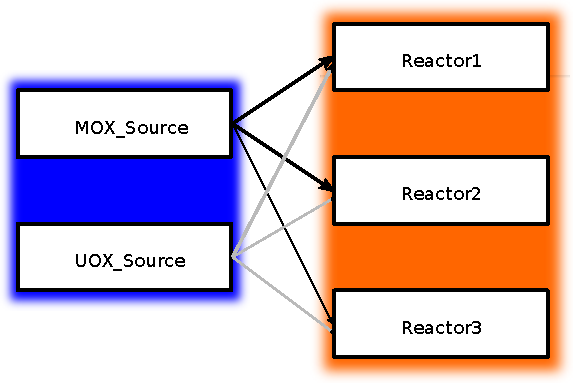
\includegraphics[width=0.55\textwidth]{./figs/fc1.pdf}
    \caption[]{\label{fig::fc1}
        Schematic illustrating the fuel cycle scenario. The thickness of the
        arrows represents the preference value and the grey color indicates that
        a material transfer is possible.}
  \end{center}
\end{figure}

In this example case \Reactor{1}, \Reactor{2}, and \Reactor{3} are deployed
sequentially over 3 time steps. Each of these has a full core when built and
requires 1 kg of fresh fuel at each subsequent time step. Both source facilities
have a capacity of 2.5 kg each time step.

The simulation begins with the following facilities: \MOXSource{}, \UOXSource{},
and \Reactor{1}. At time step 2, \Reactor{2} is deployed, followed
by \Reactor{3} at time step 3. \Reactor{1} and \Reactor{2} both are given a
stronger preference for MOX requests than \Reactor{3}. At time step
4, \Reactor{1}, \Reactor{2}, and \Reactor{3} all request to refuel with MOX. At
time step 5, \Reactor{1} changes its preference to UOX. Table \ref{table::scen1}
summarizes the reactor preferences as a function of time.

\FloatBarrier
\begin{table}
  \begin{center}
    \caption{\label{table::scen1} 
        Time sequence of reactor preferences and the total MOX requested. The MOX capacity for each time step is 2.5 kg.}
    \begin{tabular}{m{1cm}|cc|cc|cc|m{2cm}}
    \toprule
    Time step & \multicolumn{2}{c|}{\Reactor{1}} & \multicolumn{2}{c|}{\Reactor{2}} & \multicolumn{2}{c|}{\Reactor{3}} & Total MOX Requested [kg]\\
              & Fuel & Preference & Fuel & Preference & Fuel & Preference  \\
    \midrule
    1         & MOX  & 1.0 & none &     & none &     & 0.0 \\
    2         & MOX  & 1.0 & MOX  & 1.0 & none &     & 1.0 \\
    3         & MOX  & 1.0 & MOX  & 1.0 & MOX  & 0.5 & 2.0 \\
    4         & MOX  & 1.0 & MOX  & 1.0 & MOX  & 0.5 & 3.0 \\
    5         & UOX  & 2.0 & MOX  & 1.0 & MOX  & 0.5 & 2.0 \\
    \bottomrule
    \end{tabular}
  \end{center}
\end{table}
\FloatBarrier

\paragraph{Enrichment, 2 Reactors}

As pictured in Figure \ref{fig::fc2}, this scenario includes
one \textit{EnrichmentFacility} and
two \textit{BatchReactors}. The \textit{EnrichmentFacility}, denoted
as \Enrichment{}, has a designated capacity at each time step. The
two \textit{BatchReactors}, denoted as \Reactor{1} and \Reactor{2}, request a
given amount and quality of enriched uranium upon refueling.

\begin{figure}
  \begin{center}
    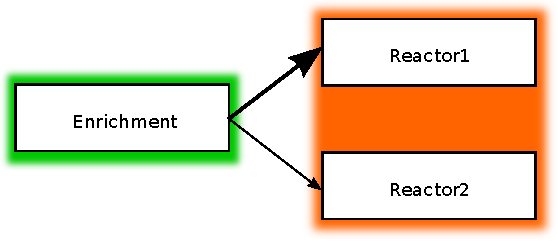
\includegraphics[width=0.55\textwidth]{./figs/fc2.pdf}
    \caption[]{\label{fig::fc2}
        Schematic illustrating the fuel cycle scenario. The thickness of the arrows represents the preference value.}
  \end{center}
\end{figure}

The \Enrichment{} facility is constrained by a constant capacity of 10 SWU per
time step. For this entire simulation, trade between \Enrichment{}
and \Reactor{1} is preferred over trade between \Enrichment{} and \Reactor{2}
with preference values of 1.0 and 0.5, respectively. The preferences are
assigned to reactors in order to provide a consistent solution using the greedy
algorithm described in \S \ref{subsect::drep}. Each reactor requests 1 kg of
enriched uranium at each time step.

Initially, both reactors are present in the simulation and have a full core of
3\% enriched uranium. On time step 1, \Reactor{1} requests uranium enriched to
5\% U-235 while \Reactor{2} requests uranium at a 3\% enrichment level. At time
step 2, \Reactor{1} reduces its enrichment request to
3\%. Table \ref{table::scen2} summarizes the reactor requests as a function of
time.

\FloatBarrier
\begin{table}
  \begin{center}
    \caption{\label{table::scen2}
        Time sequence of reactor preferences and the total SWU requested. The SWU capacity for each time step is 10.}
    \begin{tabular}{m{1cm}|cc|cc|m{2cm}}
    \toprule
    Time step & \multicolumn{2}{c|}{\Reactor{1}} & \multicolumn{2}{c|}{\Reactor{2}} & Total SWU Requested \\
              & Recipe & Preference     &     Recipe & Preference \\
    \midrule
    0         & 3\% U-235 &     & 3\% U-235 &     &  0   \\
    1         & 5\% U-235 & 1.0 & 3\% U-235 & 0.5 & 10.6 \\
    2         & 3\% U-235 & 1.0 & 3\% U-235 & 0.5 &  6.8 \\
    \bottomrule
    \end{tabular}
  \end{center}
\end{table}
\FloatBarrier

\subsubsection{Results}

To demonstrate the dynamic resource exchange implemented in \Cyclus{} relatively
small simulations may be performed. This is in part because market demands may
be independently varied from time step to time step.  Furthermore, dynamism is
demonstrated only when market demands change. Integrating results over several
time steps with the same steady state conditions and constraints does not yield
new insights into the procedure at hand.

The cases outlined in \S \ref{subsect::fcdesc} have been designed to 
provide different conditions at each point in time. This maximizes the
meaningful information produced per unit of computational effort.
The results for these cases are discussed in \S \ref{subsect::2srcs3rxts} and 
\ref{subsect::1enr2rxts}.  In each of these cases, the total \Cyclus{} run time
was $\sim$0.1 seconds and the output database size was $\sim$68 kB.

\paragraph{2 Sources, 3 Reactors}
\label{subsect::2srcs3rxts}
Initially present are the source facilities and \Reactor{1}.  \Reactor{1} has 
a preference for accepting MOX fuel over UOX.  The \MOXSource{} capacity of 2.5 kg 
is more than 
enough to handle the 1 kg of MOX requested by \Reactor{1}.  This matching may be seen
in Figure \ref{fig::2srcs3rxts-t1}.

\begin{figure}
  \begin{center}
    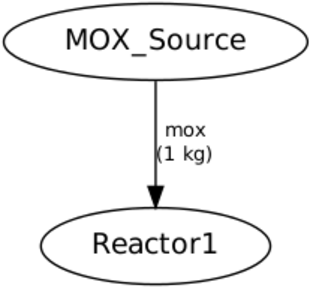
\includegraphics[height=3cm]{./figs/2_Sources_3_Reactors-t1.pdf}
    \caption[]{\label{fig::2srcs3rxts-t1}Time step 1 for the 2 Sources, 3 Reactors 
        case.}
  \end{center}
\end{figure}

Note that the resource flows in Figures 
\ref{fig::2srcs3rxts-t1}-\ref{fig::enr2rxts-t3}
have been generated automatically from \Cyclus{} output using
Cyan \cite{Carlsen2014}.  Due to this, these figures only show facility agents
which participated in a resource exchange. Other facilities may exist but are
not displayed if no resource was traded.  Thus Figure \ref{fig::2srcs3rxts-t1}
does not show the \UOXSource{} facility, even though it is present in the
simulation.  Finally in Figure \ref{fig::2srcs3rxts-t1} the \MOXSource{} only
provides the 1 kg of material requested by \Reactor{1}.  It, correctly, does not
oversupply.

\begin{figure}
  \begin{center}
    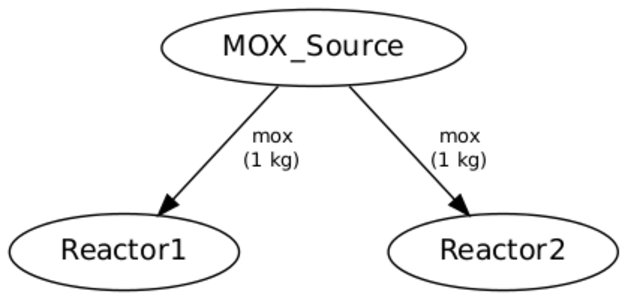
\includegraphics[height=3cm]{./figs/2_Sources_3_Reactors-t2.pdf}
    \caption[]{\label{fig::2srcs3rxts-t2}Time step 2 for the 2 Sources, 3 Reactors 
        case.}
  \end{center}
\end{figure}

At time step in 2 in this simulation, \Reactor{2} is deployed and also requests 
fuel with the preference for MOX.  Figure \ref{fig::2srcs3rxts-t2} displays
that the \MOXSource{} indeed has the required capacity to meet the requests of 
both of the reactors.  This may seem trivial at first glance but it is important 
to emphasize that the resource exchange solver was not altered in any way to handle 
both time steps 1 and 2.  Furthermore, the solver on time step 1 had no future 
knowledge that \Reactor{2} would be deployed on time step 2.  This is significantly 
different than the traditional system dynamics approach.

\begin{figure}
  \begin{center}
    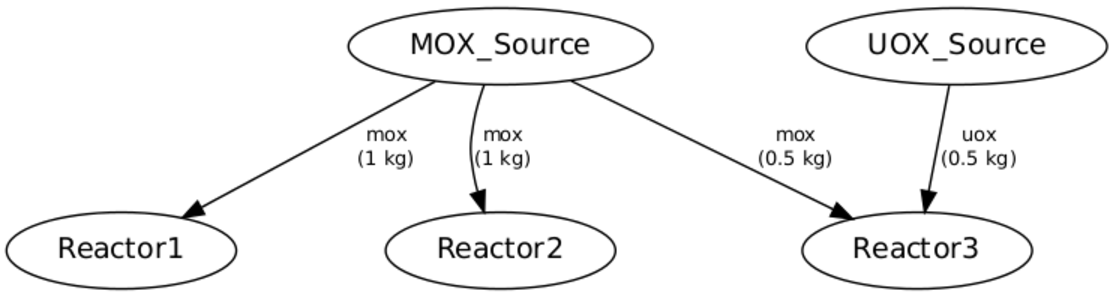
\includegraphics[height=3cm]{./figs/2_Sources_3_Reactors-t3.pdf}
    \caption[]{\label{fig::2srcs3rxts-t3}Time step 3 for the 2 Sources, 3 Reactors 
        case.}
  \end{center}
\end{figure}

On time step 3, \Reactor{3} is deployed.  This facility still prefers to accept 
MOX fuel over UOX fuel.  At this point, 3 kg of MOX are requested (1 kg from 
each facility) but the \MOXSource{} may only provide 2.5 kg.  Because of this, 
the \UOXSource{}, which has been present in the simulation since the beginning, 
now enters the exchange to make up for the missing 0.5 kg of fuel not obtainable 
from the \MOXSource{}. \Reactor{3} is selected to receive the UOX fuel rather than 
\Reactor{1} and \Reactor{2}.  These preferences are detailed in Table \ref{tab::pref-t3}.  In time step 3 because all agents tie for UOX, 
\Reactor{1} and \Reactor{2} tie for MOX, and the \Reactor{3} preference for MOX is 
less than the others, \Reactor{3} loses its full bid for MOX and must top-up with 
UOX.  This is precisely the situation displayed in Figure \ref{fig::2srcs3rxts-t3}.

\begin{table}
  \begin{center}
    \caption{\label{tab::pref-t3}Resource exchange preferences for agents on 
             time steps 3 and 4 for reactors in the 2 sources, 3 reactors case.}
    \begin{tabular}{lcc|cc}
    \toprule
          & \multicolumn{2}{c}{$t=3$} & \multicolumn{2}{c}{$t=4$} \\
    Agent & UOX & MOX & UOX & MOX\\
    \midrule
    \Reactor{1} & 0.0 & 1.0 & 2.0 & 1.0 \\
    \Reactor{2} & 0.0 & 1.0 & 0.0 & 1.0 \\
    \Reactor{3} & 0.0 & 0.5 & 0.0 & 0.5 \\
    \bottomrule
    \end{tabular}
  \end{center}
\end{table}

Finally, on time step 4 the preference of \Reactor{1} for UOX changes from 
0.0 to 2.0.  This alteration causes the tie previously present 
for UOX to be broken.  Furthermore, the value of 2.0 makes this the most 
preferred arc in the system so it is attempted to be satisfied first.  
As may be seen in Figure \ref{fig::2srcs3rxts-t4}, the \UOXSource{} capacity of
2.5 kg is more than enough to satisfy the request from \Reactor{1} for 1 kg of UOX.
Since \Reactor{1} does not diminish the capacity of the \MOXSource{} both \Reactor{2} 
and \Reactor{3} are able to obtain their first choice fuel.

\begin{figure}
  \begin{center}
    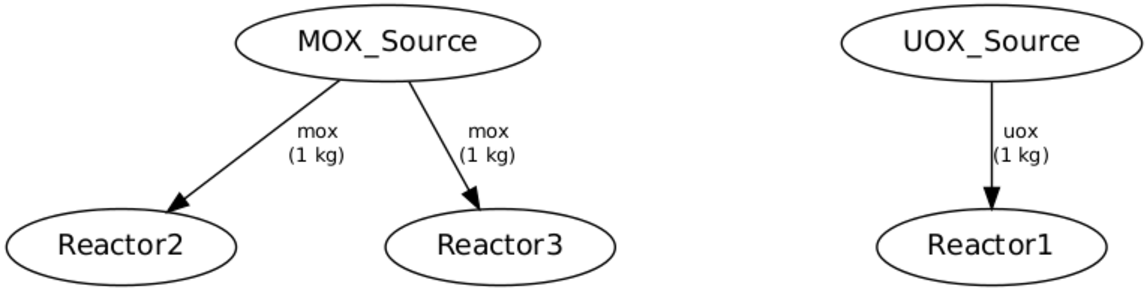
\includegraphics[height=3cm]{./figs/2_Sources_3_Reactors-t4.pdf}
    \caption[]{\label{fig::2srcs3rxts-t4}Time step 4 for the 2 Sources, 3 Reactors 
        case.}
  \end{center}
\end{figure}

This simple 2 source, 3 reactor simulation shows how the resource 
exchange can dynamically and correctly adapt to the both facility deployments and
the preferences that these agents have for requested resources.

\paragraph{Enrichment and 2 Reactors}
\label{subsect::1enr2rxts}

Initially, \Enrichment{}, \Reactor{1}, and \Reactor{2} are all present. The reactors both begin with cores composed of 3\% enriched uranium. 

\begin{figure}
  \begin{center}
    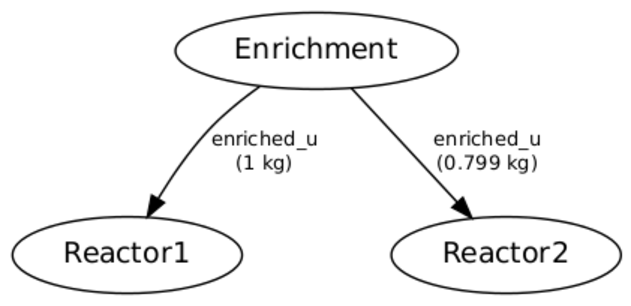
\includegraphics[height=3cm]{./figs/1_Enrichment_2_Reactor-t1.pdf}
    \caption[]{\label{fig::enr2rxts-t1}Time step 1 for the Enrichment and 2 Reactors 
        case.}
  \end{center}
\end{figure}

Figure \ref{fig::enr2rxts-t1} shows the result of the resource exchange for time
step 1.  Here the SWU capacity of \Enrichment{} is not sufficient to meet the
requests for 5\% and 3\% enriched fuel simultaneously but is enough to meet
either of them individually.  Therefore, the bid for at least one of the
reactors must be partially unmet.  Due to the preferences, the requests
of \Reactor{1} will be met first.  Thus in
Figure \ref{fig::enr2rxts-t1} \Reactor{1} receives 1 kg of 5\% enriched fuel.
However, \Reactor{2} only receives $\sim$80\% of its request for 3\% enriched
uranium.  This is not enough to run on and so this material is saved for the
future.

\begin{figure}
  \begin{center}
    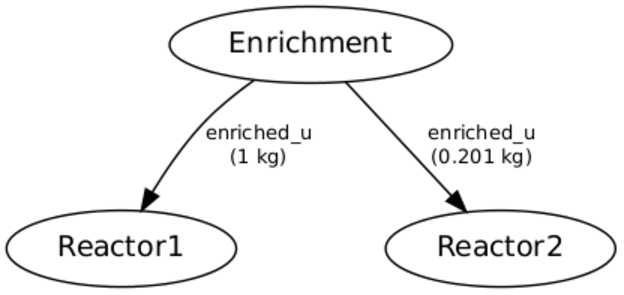
\includegraphics[height=3cm]{./figs/1_Enrichment_2_Reactor-t2.pdf}
    \caption[]{\label{fig::enr2rxts-t2}Time step 2 for the Enrichment and 2 Reactors 
        case.}
  \end{center}
\end{figure}

On time step 2, \Reactor{1} now switches from requesting 5\% enriched fuel to
requesting 3\% enriched fuel.  However, the reactor archetypes are implemented
such that if they have stored fuel from a previous time step, they will instead
only request a mass needed to create 1 kg of fuel.  Therefore, \Reactor{2} only
requests $\sim$0.2 kg from \Enrichment{}.  \Reactor{1} continues to request 1 kg
of material and this is met because the SWU capacity constraint is not exceeded.
These resource flows may be seen in Figure \ref{fig::enr2rxts-t2}.

\begin{figure}
  \begin{center}
    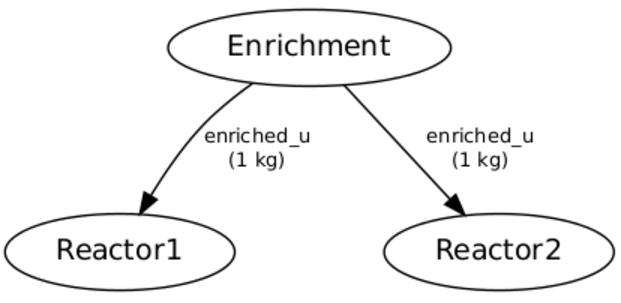
\includegraphics[height=3cm]{./figs/1_Enrichment_2_Reactor-t3.pdf}
    \caption[]{\label{fig::enr2rxts-t3}Time step 3 for the Enrichment and 2 Reactors 
        case.}
  \end{center}
\end{figure}

No further adjustments of requests were made on time step 3. Thus the results 
displayed in Figure \ref{fig::enr2rxts-t3} represent the same dynamic resource 
exchange procedure in time step 2.  The key differences here however are that 
now the system has returned to a steady state and - unlike in time step 1 - 
the SWU capacity of \Enrichment{} is enough to meet the 2 kg of 3\% enriched
fuel coming from both reactors.  Thus \Reactor{1} and \Reactor{2} each receive 
the kilogram of fuel that they request.  Without further adjustments this 
system will continue \emph{ad infinitum}.

